%\documentclass[10pt,a4paper]{article}
\documentclass[letterpaper,10pt,draftclsnofoot,onecolumn]{article}
\usepackage[letterpaper, margin=.75in]{geometry}

\usepackage{hyperref}
\usepackage{listings}
\usepackage{wasysym}
\usepackage{graphicx}

\hypersetup{
	colorlinks,
	citecolor=black,
	filecolor=black,
	linkcolor=black,
	urlcolor=black
}

\begin{document}
\begin{titlepage}
\vspace*{\fill}
\begin{center}
{\Large Tut-Tut, The IoT Rain Fall Detector Design Document}
\\[0.3cm]

{\large Team 21}
\\[0.3cm]

{\large CS 461 - Fall 2018}
\\[0.3cm]

{\large Michael Gillett, Casing and Microcontroller Lead}
\\[0.3cm]
{\large Jonathan Rohr, Data Collection and Management Lead}
\\[0.3cm]
{\large Shreyans Khunteta, UI Lead}
\\[0.3cm]

{\large November 26, 2018}
\\[1cm]

{\Large \textbf{Abstract}}
\end{center}
Tut-Tut, the IoT Raindrop Detector, is a project under the domain of the OPEnS (Openly Published Environment Sensing) Lab at Oregon State University. Tut-Tut will be able to detect a drop of any size, get an idea of the raindrop mass from the intensity at which it falls, and detect the frequency of raindrops. After Tut-Tut gathers this data, it will be able to wirelessly transmit the information to a central server and communicate it to other IoT devices around Oregon State University. The detector will have a 2 cm by 2 cm area it can sense rain in, will wake up with a single raindrop, and will stay awake as long as more rain is detected within a minute. In addition to the physical device, we will also design a browser UI to make the gathered data more readable.
\vspace*{\fill}
\end{titlepage}

\begin{center}
\section*{Glossary}
\end{center}

\quad \newline
\textbf{OPEnS Lab:} Openly Published Environmental Sensing Lab. Located at Oregon State University, this lab's goal is to develop environmental sensing devices and do research on their findings.
\newline
\newline
\textbf{CAD:} Computer-Aided Design. CAD is not a single program, but a technique used by many programs to design and simulate 3D objects that will be used in production.
\newline
\newline
\textbf{IDE:} Integrated Development Environment. Usually refers to the program being used to write and test the coded sections of the project.
\newline
\newline
\textbf{IoT:} Internet of Things. Used to describe a system made up of interconnected devices that form a network.
\newline
\newline
\textbf{Piezo Sensor:} Piezoelectric sensor. A device that uses the piezoelectric effect to measure changes in force by converting them to an electrical charge.
\newline
\newline
\textbf{MEMS Piezo Vibration Sensor:} Microelectromechanical systems sensor. Uses the piezoelectric effect to measure vibrations, but the sensor is small and its components are near microscopic.
\newline
\newline
\textbf{Accelerometer:} A device that measures vibrations from acceleration forces using electromechanical technology. It measures forces as voltages and then translates those voltages into vibration measurements.
\newline
\newline
\textbf{M0 Feather Microcontroller}: The M0 Feather is a microcontroller from Adafruit. It is thin, light and the centerpiece of our project. It will be handling all the computing for Tut-Tut.

\pagebreak

\tableofcontents
\pagebreak

\section{Introduction}
\subsection{Purpose}
This document will outline the design specifications referenced in each of the group members' Tech Reviews. We will discuss the design of the pieces, technologies, methods, and other parts that will be included in the final product. The final product may differ slightly from the specifications in this document, but it should act as a roadmap moving forward.

\subsection{Scope}
When the Tut-Tut reaches the end of its development, it will be expected to perform three major tasks and one task that will be implemented if there is time. First, it will need to be able to translate vibrations from rainfall into a voltage using its onboard vibration sensors. Second, it will transmit the collected data to the OPEnS Lab's Dropbox where it is subsequently stored into a spreadsheet in real-time. Third, it must be integrated into their existing ecosystem of sensors, Loom. Finally, if time permits, a browser UI will be used to communicate the Tut-Tut data in an easy to understand way.

\subsection{Document Overview}
First, Michael details the code we will use in our Microcontroller and describes the protective casing that will encase all components of our project. Second, Jonathan describes how we will be collecting rainfall data with sensors and how that data will be sent to our online database. Finally, Shreyans outlines what our stretch goal website would look like. The group members will be primarily responsible for all the technologies in their respective sections for the remaining time frame of the entire project.

\section{System Overview}
This product is designed to accommodate any person(s) who may want to know about rainfall metrics in their area. The sensor will provide real-time information about the size/mass of the raindrops, how frequently they are falling, and the intensity of the rainfall. These metrics could be used by meteorologist as a way to show more detailed information about the rain in the local area. They could also be used by farmers to better take care of their crop fields. Furthermore, the Tut-Tut Rainfall Detector will link into the OPEnS lab's larger ecosystem of environmental devices and sensors, known as Loom. The data Tut-Tut collects will be stored in a Google Sheets database for analysis.

\section{System Architecture}

\subsection{Code Design}
This section outlines the flow of the code flashed onto the microcontroller. 
\\
\\
We will be using an Adafruit Feather M0 microcontroller with Wi-Fi capability. The code that we will use can be divided into two phases: Initialization and Loop. The initialization section will set up all the necessary pins as soon as the device is booted, such as the LED and the analog pin used by the sensor. The looping portion of the code will run continuously, record the necessary data metrics, and upload them to the central server.
\\
\\
Once we test the sensor pieces and can record an accurate output of voltage (about a 1\% error), we will have an accurate threshold of voltage that will constitute a raindrop. In the main loop, we will first check the state of the sensor. If the voltage read is above our derived value, the program flow will enter an if-statement that will take care of the uploading. For good measure, we will have a delay function at the end of the loop to avoid overloading the buffer and losing our data.\cite{Knock} 

\subsection{Casing Design}
We have not yet done a model of Tut-Tut, but we do have a few expectations of what it should contain. First, we want the final product to be portable and able to be moved from place to place. To accomplish this we will need room in the casing for a battery, our microcontroller, and the sensor. Since the device will be out in rain, the casing containing the electronics will need to be weatherproof. The shape of Tut-Tut will likely be a 2 cm by 2 cm disk-shaped area on the top for raindrops to fall on, with a heavier base containing the hardware. Figure 1 shows what Tut-Tut might look like at the end of production given these specifications.
\newline

\begin{center}
Figure 1: A basic drawing of what Tut-Tut will resemble when complete
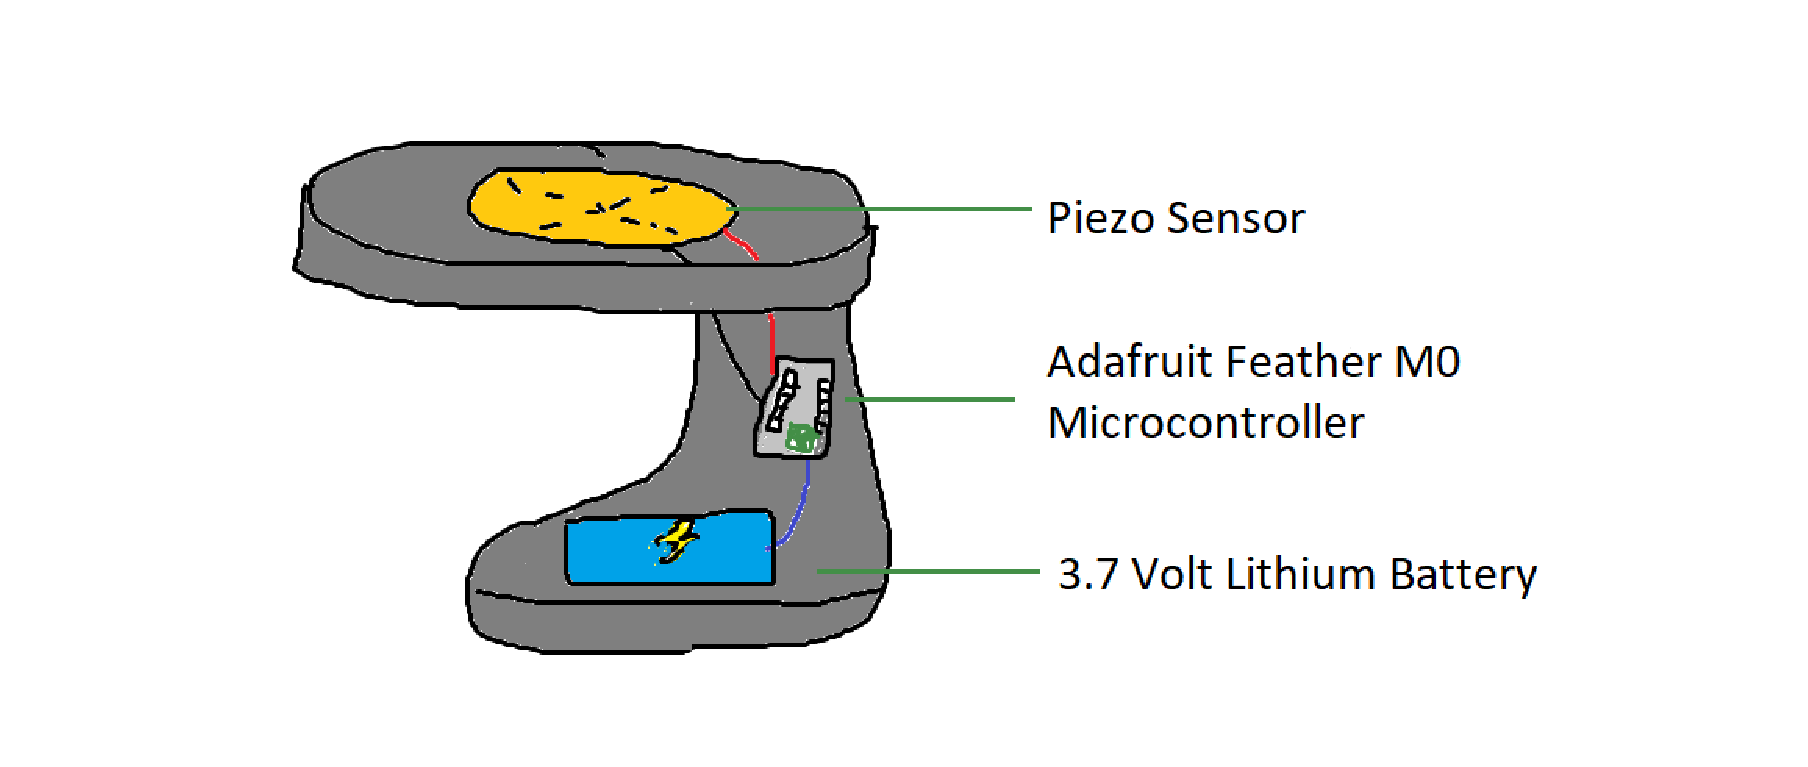
\includegraphics[width=.8\textwidth]{TutTutFirstDraft.eps}
\end{center}

\subsection{Design Rationale}
Each of the pieces of Tut-Tut had to be chosen specifically regarding the purpose of the final product. Trade-offs were (or will be) made on both the sensor and microcontroller pieces. For the microcontroller, we had the option of a basic board, one with Wi-Fi capability, and one with Long-Range Radio capability. We chose the Wi-Fi model because of the constant connection and reliable transfers of data. The sensors available to us are a piezo, a MEMS, and an accelerometer. These devices are all similar in usage and will only change the specific design of the 3D-printed casing depending on which is chosen.


\section{Data Design}

\subsection{Data Collection}
Tut-Tut will use sensors to register vibrations from raindrops. Using data gathered from the sensors, it will determine the size, density, mass, and frequency rate of these raindrops as they fall. We will be using the Piezo Vibration Sensor and the Piezo Element to accomplish these tasks. 
\\
\\
The Piezo Vibration Sensor is a MEMS sensor which uses the piezoelectric effect to detect vibrations. It has dimensions of around 1 cm wide and 2 cm long. It has a high voltage sensitivity of 1 V/g at its baseline and 6 V/g at its resonance. The sensor generates AC and voltage when the thin film gyrates. These voltages can help determine the impact velocity and mass of the raindrops.
\\
\\
The Piezo Element is a basic sensor that also uses the piezoelectric effect to detech vibrations. Raindrops impacting the flat sensor will generate voltage that will be used to determine their impact velocity and mass. The two sensors perform the same task in different ways, so they each will be tested to determine which one will work best for Tut-Tut.

\subsection{Data Management}
Tut-Tut will be gathering data in the field. This means no one will be around to monitor its results immediately. All of the data that is collected by the sensors above will have to be sent wirelessly, in real-time, to an internet hub. We will use the PushingBox to Google Sheet Pipeline that has already been discovered by the OPEnSLab.\cite{PushingBox} As our Arduino Board gathers data from the sensors, it will make GET requests to a PushingBox Scenario using the data to be sent as URL arguments. The PushingBox Scenario formats the data and sends it as URL arguments in its own GET request to the Google Sheet. The Google Sheet will then parse through and display the data. PushingBox currently only supports 1000 requests per day per user. This means that Tut-Tut will only be able to send a string of data once every two minutes.

\section{Human Interface Design}
Currently our scope for the UI is limited. All the information and relevant performance metrics will appear as an Excel spreadsheet you can access through a website link. However, our stretch goal is to create a fully functioning user interface that the user can navigate. This fully functional user interface will be on a website that looks fairly similar to the OPEnS lab website (http://www.open-sensing.org/). 
\newline

\begin{center}
Figure 2: The current OPEnS Lab website. Tut-Tut's website will resemble this in aesthetic.\cite{OPEnSLab}
\includegraphics[width=.9\textwidth]{openslab.eps}
\end{center}

\subsection{Overview of User Interface}
This user interface will be built with programming languages such as HTML, CSS and JavaScript. The user interface design is still in progress and it is important to stress that this is a stretch goal. However, we want the final appearance of it to be visually appealing and engaging, and to be be usable and understandable by any educated user, and not just the OPEnS lab staff and students.

\subsection{Screen Images}
The images on the screen will be pictures of OPEnS staff and OPEnS lab projects, such as Tut-Tut itself. It will remain tasteful and aesthetically pleasing, and will incorporate Oregon State logos as well. We will have it try to remain the OPEnS lab webpages themselves.

\subsection{Screen Objects and Actions}
We may implement some minor transitions between pages to make the site look more appealing to the user. However we are not going to use JavaScript effects for the sake of JavaScript effects. We want every transition we do to be for the ultimate comfort and ease of the user. Our design for this will flesh out as the project goes forward, as this is still our stretch goal.

\pagebreak

\section{Conclusion}
This document will generally outline the remainder of Tut-Tut's production and give us a road map in which to reference as needed. First, the code will constantly loop checking for forces read from the Piezo above our calculated threshold, and take appropriate action when an exerted force does cross it. Next, we will have all of our hardware components contained in a waterproof shell that is bottom-heavy with a 2x2 cm disk-shaped surface area to measure the rain drops as they hit. The resulting voltages will be translated into meaningful data and sent through the PushingBox to Google Sheet Pipeline. Finally, if time permits, we will create a UI based off the OPEnS Lab website. It will be easily navigable by any user and will have performance metrics that Tut-Tut will be tracking (raindrop size, intensity and frequency rate). If we are unable to meet this stretch goal, the UI will simply be a Google Sheets document with all the relevant performance metrics.

\pagebreak
\bibliography{reference}
\bibliographystyle{ieeetr}

\end{document}